\documentclass[12pt,twoside]{article}

% *** Set page dimensions ***
\raggedbottom
\parindent=0in
%\setlength{\topmargin}{-0.5in}
%\setlength{\oddsidemargin}{0.1875in}
%\setlength{\evensidemargin}{0in}
%\setlength{\textheight}{8.5in}
%\setlength{\textwidth}{6.225in}
%\addtolength{\oddsidemargin}{-0.7in}
%\addtolength{\evensidemargin}{-1.2in}
%\setlength{\oddsidemargin}{-0.2in}
%\setlength{\evensidemargin}{-0.2in}
%\addtolength{\textwidth}{1.4in}
%\addtolength{\topmargin}{-.875in}
%\addtolength{\textheight}{2.00in}

% *** Packages ***
\usepackage{alltt}
\usepackage{tocloft}
\usepackage{graphicx}
\usepackage{lscape}
\usepackage{amssymb}
\usepackage{float}
\usepackage{amsmath}
\usepackage{gensymb}
%\usepackage{subfigure}
\usepackage{lscape}
\usepackage{epsfig}
\usepackage{enumerate}
\usepackage{multicol}
\usepackage{fancyhdr}
\usepackage{epstopdf}
\usepackage{hyperref}
\usepackage{listings}

% *** Table of contents and Sectioning *** 
\setcounter{secnumdepth}{0}
\setcounter{tocdepth}{5}

% *** Table of contents and Sectioning *** 
\newcommand{\next}{\addtocounter{enumi}{9} \item}
\newcommand{\now}[1]{\setcounter{enumi}{#1}}
\newcommand{\Z}{\mbox{\sf Z\hspace{-1.5mm}Z}}
\newcommand{\R}{\mbox{\rm I\hspace{-0.75mm}R}}
\columnsep=0.75in

% *** Shortcuts for syntax ***
\newcommand{\ds}{\displaystyle }
\newcommand{\vsc}{\vspace{4mm}}
\newcommand{\dd}[1]{\frac{d}{d{#1}} \,} 
\newcommand{\ddx}{\frac{d}{dx} \,} 
\newcommand{\ddy}{\frac{d}{dy} \,} 
\newcommand{\ddz}{\frac{d}{dz} \,} 
\newcommand{\dydx}{\frac{dy}{dx} \,} 
\newcommand{\dydt}{\frac{dy}{dt} \,} 
\newcommand{\dfdx}{\frac{df}{dx} \,} 
\newcommand{\ddt}[1]{  \frac{d{#1}}{dt} }
\newcommand{\pp}[2]{  \frac{\partial{#1}}{\partial {#2}} }
\newcommand{\zx}{\frac{\partial z}{\partial x} \,}
\newcommand{\zy}{\frac{\partial z}{\partial y} \,}
\newcommand{\limh}{\lim_{h \rightarrow 0} \;}
\newcommand{\diff}{\frac{d}{dx} \,}
\newcommand{\de}{\Delta}
\renewcommand{\thesection}{\Roman{section}}
\newcommand{\bfr}{\begin{flushright}}
\newcommand{\efr}{\end{flushright}}
\newcommand{\dx}{\frac{\partial f}{\partial x} \,}
\newcommand{\dy}{\frac{\partial f}{\partial y} \,}
\newcommand{\p}{\partial}
\newcommand{\vi}{\vec{i}}
\newcommand{\vj}{\vec{j}}
\newcommand{\vk}{\vec{k}}
\newcommand{\lan}{\left\langle}
\newcommand{\ran}{\right\rangle}
\newcommand{\reading}[1] { {\em Reading: #1}}
\renewcommand{\Pr}{ \mbox{Pr}}

% *** Commands related to textbook references
\newcommand{\problem}{{\bf Problem.} }

% *** Footnoting with symbols ***
\long\def\symbolfootnote[#1]#2{\begingroup%
\def\thefootnote{\fnsymbol{footnote}}\footnote[#1]{#2}\endgroup}

% *** Defining a boxed note ***
\floatstyle{boxed}
\newfloat{noteinbox}{htb}{loa}
\newenvironment{boxnote}{\begin{noteinbox}[H]}{\end{noteinbox}}

\newcommand{\Question}{ {\bf Question: }  }
\newcommand{\Example}[1]{ {\bf Example: } {\em #1} }
\newcommand{\ExampleCont}[1]{ {\em #1} }

% *** Define the boxed Week #/summary at the beginning/end of every chapter ***
\newcommand{\sectionbox}[1]{% 
\begin{tabular}{|p{6in}|}%
\hline%
\ \\ %
{\Large {\bf {#1}}}  \\%
\ \\%
\hline%
\end{tabular}}

% *** Shortcuts *** 
\newcommand\goals{\large {\bf {Goals:}}}
\newcommand\setfont{ }

% *** Week commands: overwritten in each notes file
\newcommand{\Week}{Null-InPreambleCommon}
\newcommand{\WeekTitle}{Null-InPreambleCommon}
\newcommand{\Course}{MNTC P04}
\newcommand{\SetNum}{1 }
\newcommand{\topic}[1]{
\newpage
\setcounter{page}{1}
\fancyhead[LE,RO]{#1 - \thepage}
}

% *** Setup Latex for the large version of the files ***
%\usepackage[landscape]{geometry}
\usepackage[letterpaper,landscape,hmargin={.8in,.8in},vmargin={1in,0.2in}]{geometry}

% Remove paragraph indents
\setlength{\parindent}{0pt}

% Spacing at the top for the header is too large by default
\setlength{\voffset}{-5ex}

% **** RENEW SCALING COMMANDS HERE ****
% *** Text in boxes ***
\renewenvironment{boxnote}{\begin{noteinbox}[H] \huge}{\end{noteinbox}} 

% *** Chapter lead in/summary boxes ***
\renewcommand{\sectionbox}[1]{% 
\begin{tabular}{|p{9.5in}|}%
\hline%
\ \\ %
{\huge {\bf {#1}}}  \\%
\ \\%
\hline%
\end{tabular}}

% *** 'Section'' commands, which are sometimes used for spacing
% From http://zoonek.free.fr/LaTeX/LaTeX_samples_section/0.html
\makeatletter
 \renewcommand\section{\@startsection {section}{1}{\z@}%
                                    {-3.5ex \@plus -1ex \@minus -.2ex}%
                                    {0.3ex \@plus.2ex}%
                                    {\setfont\bf}}

 \renewcommand\subsection{\@startsection {subsection}{1}{\z@}%
                                    {-3.5ex \@plus -1ex \@minus -.2ex}%
                                    {0.3ex \@plus.2ex}%
                                    {\setfont\bf}}

% *** 'Goals' should be larger in the overheads ***
\renewcommand\goals{\huge {\bf {Goals:}}}
\renewcommand\setfont{\huge }

\thispagestyle{empty}

\setfont 

\newcommand{\WeekTitleOne}{Derivatives - Foundations}
\newcommand{\WeekTitleTwo}{Derivatives - Linearization and Applications}
\newcommand{\WeekTitleThree}{Derivatives - Modeling}
\newcommand{\WeekTitleFour}{Integrals - Foundations}
\newcommand{\WeekTitleFive}{Integrals - Techniques}
\newcommand{\WeekTitleSix}{Integrals - Modeling}
\newcommand{\WeekTitleSeven}{Differential Equations - }
\newcommand{\WeekTitleEight}{Differential Equations - }
\newcommand{\WeekTitleNine}{Differential Equations - }
\newcommand{\WeekTitleTen}{Linear Algebra - }
\newcommand{\WeekTitleEleven}{Linear Algebra - }
\newcommand{\WeekTitleTwelve}{Linear Algebra - }



\newcommand{\Fe}{ F_{\mbox{ext}} }
\newcommand{\Fg}{ F_{\mbox{grav}} }

\begin{document}
\setfont
\pagestyle{fancy}
\renewcommand{\Week}{8 }
\renewcommand{\WeekTitle}{\WeekTitleEight }

\fancyhead[LE,RO]{Week \Week}  % default, usually only for first page
\fancyfoot{}
\sectionbox{Week \#\Week: \WeekTitle}

\vspace{5mm}
\goals
\begin{itemize}
\item Express real world situations in terms of second order linear
  differential equations.
\item Describe the difference between homogeneous and nonhomogeneous
  second order linear differential equations.
\item Use MATLAB to solve linear and nonlinear second order
  differential equations, both homogeneous and nonhomogeneous.
\end{itemize}
\vspace{5mm}

\newpage

\topic{Generating Numerical Solutions with MATLAB}
\subsection*{Generating Numerical Solutions with MATLAB}

\problem Search for ``ordinary differential equations'' in MATLAB help.  \vsc
\vsc

What form of differential equation does MATLAB assume we have?

\vsc
\vsc


\newpage

Note that MATLAB has many different differential equation solvers. If
using MATLAB after this course, you may have to do some reading to
identify the properties of the equation you have, and what the most
appropriate solving tool is.

\problem Which of the solvers is recommended as a ``first try''
solver?

\vsc
\vsc

\newpage

\subsection*{ode45}
The first solver to reach for in MATLAB is \verb#ode45#.  To run it, we need
\begin{itemize} 
\item the DE function {\bf in form $\displaystyle \frac{dy}{dt} = f(t, y)$};
\vfill
\item the time span for the solution/simulation, $[t_0, t_{\mbox{end}}]$; and
\vfill
\item the initial condition ($y(t_0))$
\vfill
\end{itemize}

\problem What will \verb#ode45# compute for us, given that
information?
\vfill
\vfill

\newpage

\topic{Example - Temperature Model}
\subsection*{Temperature Model - Newton's Law of Heating and Cooling}

The temperature of an object, $y$, changes at a rate proportional to
the temperature difference between object, $y$, and its environment,
$T_{\mbox{ext}}$.

\problem Translate this law into a mathematical statement.

\vfill Solution interpretation: a {\bf solution} to a differential
equation is the same as a {\bf prediction}.  \vspace{1.5in}

\newpage 

{\bf In MATLAB}

$$\frac{dy}{dt} = -k (y - T_{\mbox{ext}})$$


\begin{verbatim}
% Define temp DE in the form dy/dt = f(t, y)
% and set other constants
k = 0.7;  % /min

T_ext = 20; % external/environment temp

DE = @(t, y)   -k (y - T_ext);

\end{verbatim}

\newpage

\subsection*{Example - Step 2}
\begin{verbatim}
% Solve based on initial condition
y0 = 100;  % initial temperature

tspan = [0, 30];  % interval for solution

[t, y] = ode45(DE, tspan_, y0);

plot(t, y);
\end{verbatim}

\newpage

To decipher and work with the output, it is critical that you
understand what MATLAB provides.  
\begin{itemize}
\item The final values of \verb#t# and \verb#y# are 
\vfill
\item \verb#t# starts at
\vfill
\item \verb#t# ends at
\vfill
\item \verb#y# starts at
\vfill
\end{itemize}

\newpage

\subsection*{Basic Process}
How does MATLAB do it?
\vfill
\vfill

\newpage

\topic{Second-Order Linear Equations - Spring System Intro}
\section*{Second-Order Linear Equations - Spring System}

So far we have seen examples of {\bf first-order DEs}, or equations
with first derivatives of some unknown function.  

In the following examples, we will expand our study to differential
equations with {\bf second or higher derivatives}.

One classic source of differential equations of this type comes from
analyzing the forces on a block at the end of a spring.
\begin{center}
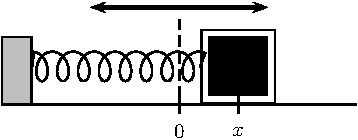
\includegraphics[width=0.5\linewidth]{graphics/notes_08_block}
\end{center}
\newpage
\begin{center}
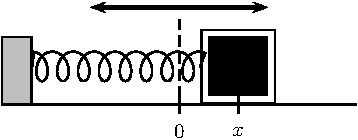
\includegraphics[width=0.4\linewidth]{graphics/notes_08_block}
\end{center}

While the mathematics behind this simple system will be very
interesting in their own right, we should also note at the outset that
the simple spring/mass model can be applied to a wide variety of
not-so-obviously related real-world problems.

\begin{center}
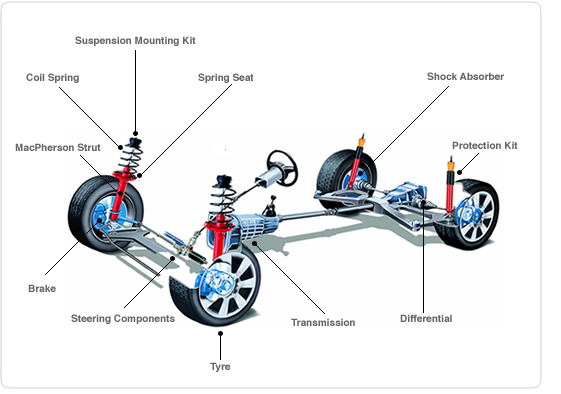
\includegraphics[width=0.30\linewidth]{graphics/notes_08_SpringSystemCar}
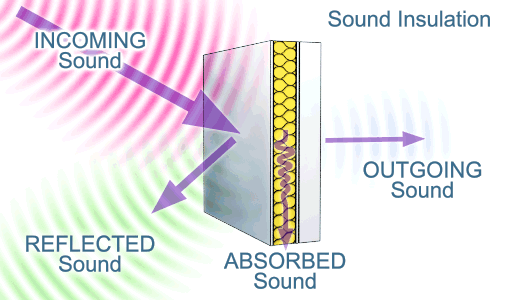
\includegraphics[width=0.30\linewidth]{graphics/notes_08_Sound-Attenuation} \\
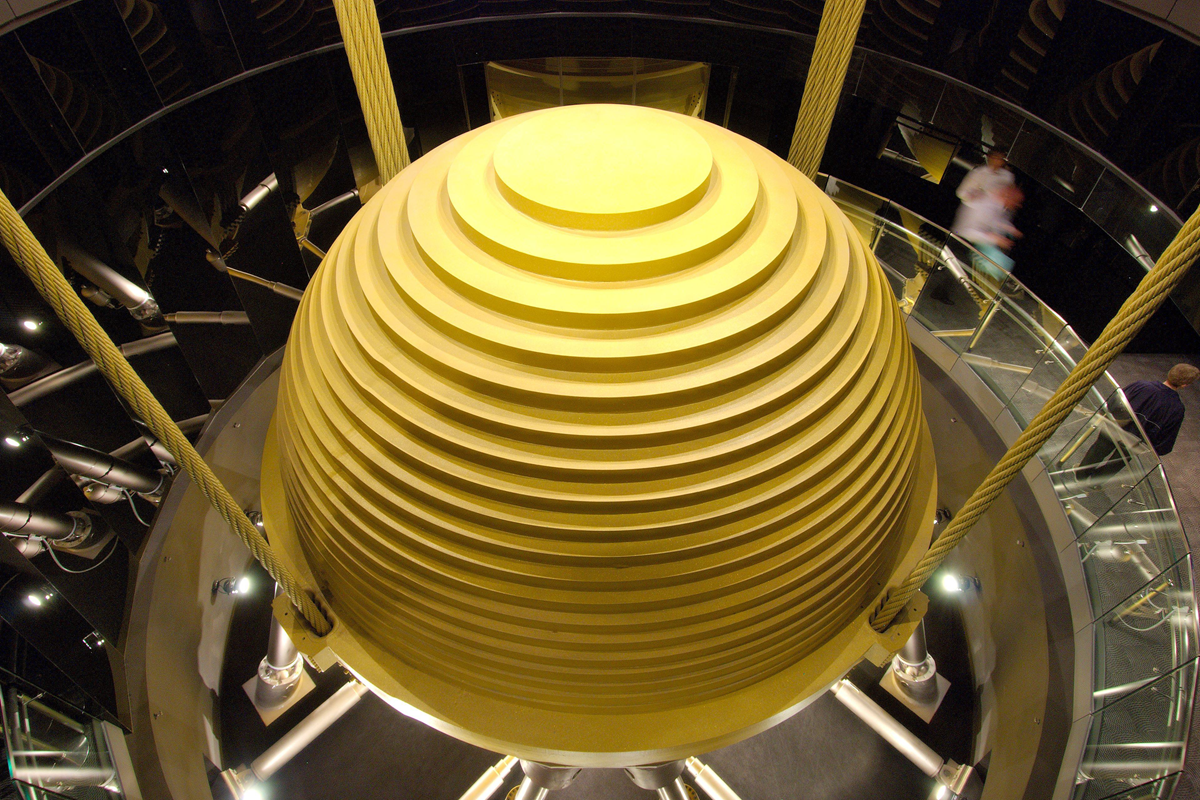
\includegraphics[width=0.30\linewidth]{graphics/notes_08_Tuned_Mass_Damper_atop_Taipei_101_-_27_March_2008}
\end{center}

\newpage

\topic{Spring System Analysis}
\subsection*{Spring System Analysis}

\begin{center}
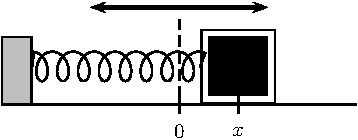
\includegraphics[width=0.5\linewidth]{graphics/notes_08_block}
\end{center}

\problem In this system, how would you describe $x$ in words?

\newpage
\begin{center}
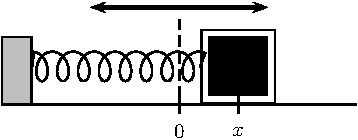
\includegraphics[width=0.35\linewidth]{graphics/notes_08_block}
\end{center}
\problem Draw a free-body diagram for the mass.  Indicate the magnitude of the forces, assuming 
\begin{itemize}
\item the mass of the block is $m$ kg, and
\item the spring constant (in $N/m$) is
  given by the constant $k$.
\end{itemize}

\newpage
\begin{center}
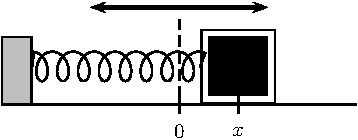
\includegraphics[width=0.35\linewidth]{graphics/notes_08_block}
\end{center}
Let us work with our intuition about this system before beginning the mathematics.

\problem If the spring is very stiff, is $k$ large or small?  \vfill

\newpage 
\begin{center}
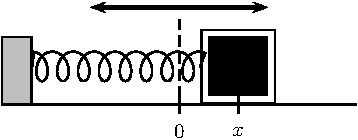
\includegraphics[width=0.35\linewidth]{graphics/notes_08_block}
\end{center}

{\bf Definition:}: {\em Period} is the length of time to
complete one full cycle/oscillation.  \vspace{0.2in}

\problem If we increase the stiffness of the spring, do you expect the
{\em period} of the oscillations to increase or decrease?  Why?

\vfill

If we increase the mass, do you expect
the \emph{period} of the oscillations to increase or decrease? Why?

\vfill

\newpage
\begin{center}
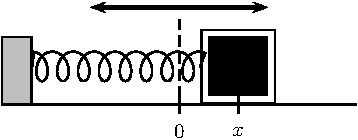
\includegraphics[width=0.35\linewidth]{graphics/notes_08_block}
\end{center}

\problem If we know $k$ and $m$, and assume that damping is
negligible, should we be able to determine the exact period of the
oscillations?  \vfill


\vfill

From the work so far, can we easily find the formula for the period?

\vfill

\newpage
\begin{center}
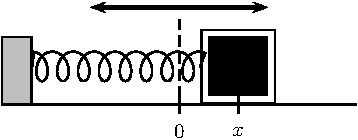
\includegraphics[width=0.35\linewidth]{graphics/notes_08_block}
\end{center}

The spring system is an excellent introduction to higher-order differential equations because 
\begin{itemize}
\item we all have an intuition about how it \emph{should} work physically,
\item the mathematics and physics are simple, and
\item there's no obvious way to predict critical features (e.g. the
  period) from the given information.
\end{itemize}
We clearly need some new tools!

\newpage
\topic{Spring System as a DE}
\subsection*{Spring System as a DE}
\begin{center}
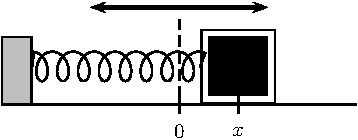
\includegraphics[width=0.35\linewidth]{graphics/notes_08_block}
\end{center}

\problem Use Newton's second law, $F = ma$, to construct an equation
involving the position $x(t)$.  \vfill

What order of differential equation does $F=ma$ produce for this
spring/mass system?

\vspace{1.3in}

\newpage

To simplify matters temporarily, let us assume that both
  $k = 1 $ N/m and $m = 1$ kg. 

  \problem Rewrite the previous differential equation using those
  constants.  \vspace{1.5in}

  This differential equation invites us to find a function $x(t)$
  whose second derivative is its own negative.  What function(s) would
  satisfy that?  \vfill

\newpage

\problem Having found two (and more) solutions to the differential
equation for the spring/mass system, how does this family of solutions
map back to the spring system?

\begin{center}
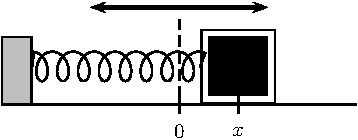
\includegraphics[width=0.4\linewidth]{graphics/notes_08_block}
\end{center}

\vfill

Is our solution an exact or a numerical solution?
\vspace{1.3in}


\newpage


\topic{Mechanical Vibrations - Spring-Mass Wystem}
\section*{Mechanical Vibrations - Spring-Mass System}

We now consider an extension to the spring/mass system.

Consider a mass $m$ hanging on the end of a vertical spring; the
spring has a naturally stretched length corresponding to $x=0$.

We have now added a damper, which exerts a force proportional to the
velocity of the oscillating mass.


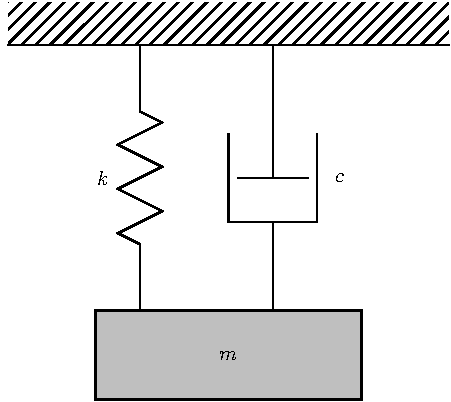
\includegraphics[width=0.4\linewidth]{graphics/notes_08_hanging_mass}

\newpage

\problem Using Newton's second law, build a differential equation that
governs the system.

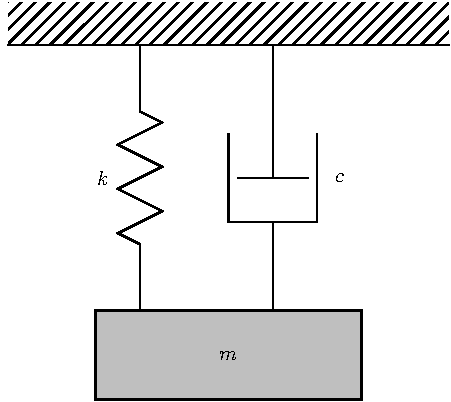
\includegraphics[width=0.35\linewidth]{graphics/notes_08_hanging_mass}


% \begin{itemize}
% \item Gravity acts downward and has a magnitude of $mg$ where $g$ is the
%   acceleration due to gravity; $F_g = mg$.
% \item The spring acts upward and, by Hooke's law, has a magnitude proportional
%   elongation.  If $y$ represents the displacement of the mass from the
%   equilibrium position, then $F_s = -k(\ell +y)$.
% \item Assuming that possible damping forces (i.e.\ a dashpot) are directly
%   proportional to the velocity of the mass, we have $F_d = - cy'$.
% \item There may be an external driving force $F(t)$.
% \end{itemize}
% Summing the forces, we find that $m y'' = F_g + F_s + F_d + F(t) = mg -k(\ell
% +y) -cy' + F(t)$.  At equilibrium, we have $mg = k\ell$ so the standard form of
% the equation is
% \[
% y'' + \tfrac{c}{m} y' + \tfrac{k}{m} y = \tfrac{1}{m} F(t) \, . 
% \]


\newpage
\problem Consider a system with a mass of $0.5 \; \text{kg}$ with
spring constant $k = 2 \; \text{N} \cdot \text{m}^{-1}$, with a
damping coefficient of $c = 0.5$ N/(m/s).  Assume the mass is
displaced $0.4 \; \text{m}$ from equilibrium and released.

\problem Write the differential equation dictates the motion of the
mass.

\vspace{1in}

Can we find an easy solution to this differential equation as we did with the undamped
case?
\vfill


Can MATLAB be used to build a numerical solution for the differential
in its current form?

\vfill

\newpage


\topic{Converting Higher-Order DEs to 1st Order Systems}
\subsection*{Converting Higher-Order DEs to 1st Order Systems}
To solve a higher-order DE using MATLAB, we need to convert it first
into a larger {\bf first-order system} of differential equations.


\vspace{0.3in}
Notation: In this section, 
\begin{itemize} 
\item vectors with be written with vector hats, e.g.
  $\vec{w}, \vec{y}$,
\item elements of a vector will be noted with subscripts, e.g. $w_1$,
  $y_2$, and
\item other scalars will be in lower-case, e.g. $c$, $\lambda$.
\end{itemize}

\newpage

\begin{minipage}[t]{0.4\linewidth}
\vspace{0pt}
Damped Spring DE:

$$ m x'' = -c x' -kx $$
\end{minipage}
\begin{minipage}[t]{0.6\linewidth}
\vspace{0pt}
\begin{center}
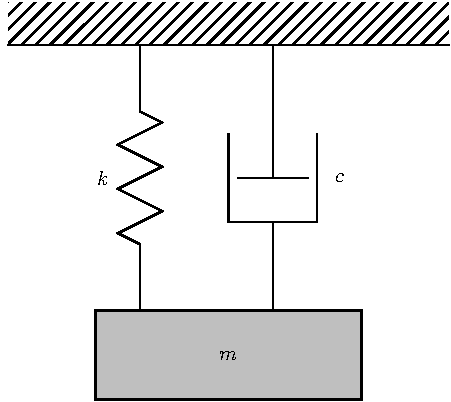
\includegraphics[width=0.5\linewidth]{graphics/notes_08_hanging_mass}
\end{center}
\end{minipage}

\problem For the spring/mass DE, define a new vector of 2 variables,
$\vec{w}$, that will allow the conversion of the second-order system
to a first-order system.

\vfill

Also see the MATLAB help menu entry on ``Ordinary Differential
Equations'', referring to ``Higher Order ODEs''.

\newpage
$$ m  x'' = -c x' -kx $$
\problem Define the derivative, $\ds \frac{d \vec{w}}{dt}$, in terms
of $\vec{w}$ itself, making use of the DE as necessary.

\vfill
\vfill

This is now a {\bf first-order system} of differential equations.  \\
The variable we are most interested in for this example is $w_1 = x$,
the {\em position} of the mass.

\newpage

\topic{MATLAB Function Files}
\subsection*{MATLAB Function Files}

Our differential equation is now sufficiently complicated that writing
it out in one line is difficult.  We will need another MATLAB tool to
proceed: a MATLAB function file.


{\bf Syntax} A MATLAB function file
\begin{itemize}
\item has as its first line the form \\
\verb#function ret = f(....)# 
\item \verb#ret# is the name of the {\bf return variable} and must be
  defined before the end of the function;
\item \verb#f# should be the same as the filename, with the \verb#.m# extension;
\item the \verb#....# can be any list of input variables.
\end{itemize}

\newpage
\problem Define a new {\bf MATLAB function \texttt{.m} file} called
\verb#hypotenuse# that takes in two lengths, \verb#a# and \verb#b#,
and returns the length of the hypotenuse for a right-angle triangle
with side lengths $a$ and $b$.

\newpage
\problem Define a new {\bf MATLAB function \texttt{.m} file} called
\verb#springDE# which computes the derivative of
$\ds \frac{d \vec{w}}{dt}$.

\begin{minipage}[t]{0.4\linewidth}
\vspace{0pt}
$$ m x'' = -c x' -kx $$
\end{minipage}
\begin{minipage}[t]{0.6\linewidth}
\vspace{0pt}
\begin{align*}
  \frac{dw_1}{dt} & = w_2 \\
  \frac{dw_2}{dt} & = \left(\frac{1}{m}\right) (-c w_2 - k w_1)
\end{align*}
\end{minipage}



\newpage 
\problem Write a MATLAB script that graphs the solution
(i.e. predicted motion) for the system described earlier:

A system with a mass of $0.5 \; \text{kg}$ with spring constant
$k = 2 \; \text{N} \cdot \text{m}^{-1}$, with a damping coefficient of
$c = 0.5$ N/(m/s).  Assume the mass is displaced $0.4 \; \text{m}$
from equilibrium and released.

Include the graphical output from MATLAB on the next page.

\newpage
\hfill
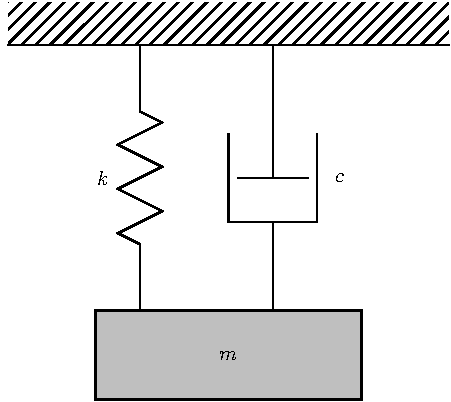
\includegraphics[width=0.3\linewidth]{graphics/notes_08_hanging_mass}


\newpage
\topic{Unforced Spring/Mass System - Patterns of Behaviour}
\subsection*{Unforced Spring/Mass System - Patterns of Behaviour}

Using MATLAB, we can now easily study the impact of different masses,
spring constants, or damping strength on the behaviour of a
spring/mass system.

\begin{minipage}[t]{0.4\linewidth}
\vspace{0pt}
Damped Spring DE:

$$ m x'' = -c x' -kx $$
\end{minipage}
\begin{minipage}[t]{0.6\linewidth}
\vspace{0pt}
\begin{center}
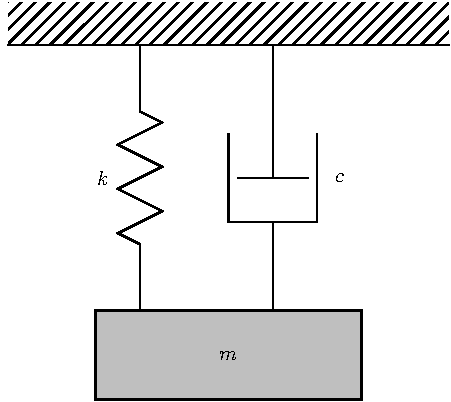
\includegraphics[width=0.5\linewidth]{graphics/notes_08_hanging_mass}
\end{center}
\end{minipage}

\newpage

A famous result in physics captures important differences in behaviour
depending on the relationship between $c$, $k$ and $m$.
\begin{itemize}
\item $c$ is 0, the system will be {\bf undamped};
\item $c$ is {\bf less} than $\sqrt{4km}$, the system will be {\bf under-damped};
\item $c$ is {\bf equal} to $\sqrt{4km}$, the system will be {\bf
    critically damped};
\item $c$ is {\bf greater} than $\sqrt{4km}$, the system will be {\bf
    over-damped};
\end{itemize}

\problem Using a spring constant of $k = 25$ N/m and mass $m = 1$ kg,
find the critical damping level.

\newpage
\problem Use MATLAB to obtain graphs for all four spring/mass cases.

  \begin{minipage}[h]{0.475\linewidth}
    \begin{center}
      
   \vspace{0pt} 
   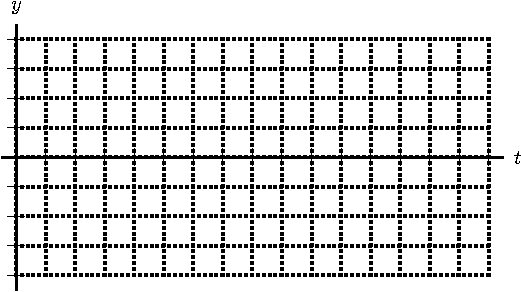
\includegraphics[width=0.9\linewidth]{graphics/notes_08_spring_mass_axes}\\
Undamped 

\hrulefill

   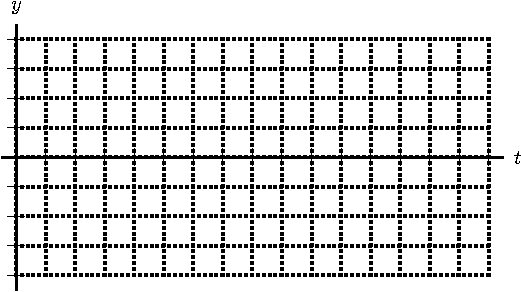
\includegraphics[width=0.9\linewidth]{graphics/notes_08_spring_mass_axes}\\
Critically Damped
    \end{center}
  \end{minipage}
  \begin{minipage}[h]{0.475\linewidth}
    \begin{center}
      
   \vspace{0pt} 
   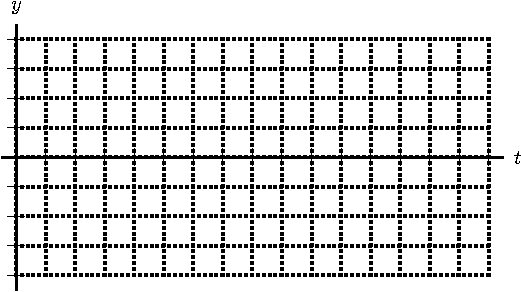
\includegraphics[width=0.9\linewidth]{graphics/notes_08_spring_mass_axes}\\
Under-Damped  

\hrulefill

   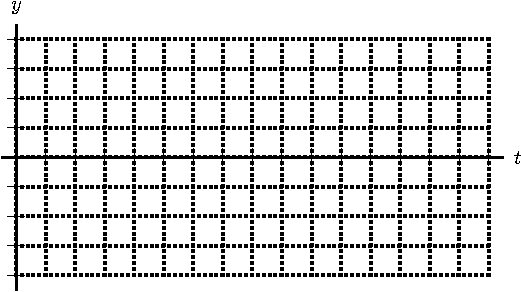
\includegraphics[width=0.9\linewidth]{graphics/notes_08_spring_mass_axes}\\
Over-Damped
    \end{center}
  \end{minipage}

\newpage
\topic{Spring/Mass with Periodic External Forces }
\subsection*{Spring/Mass with Periodic External Forces }

We now add another component to our spring system model: \\{\bf
  external forces}.

 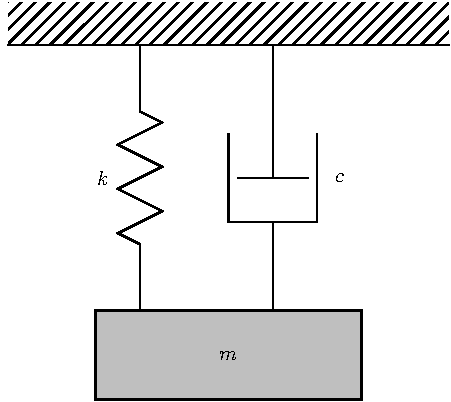
\includegraphics[width=0.25\linewidth]{graphics/notes_08_hanging_mass}

 \problem Write out the DE for the position of the mass, given the
 addition now of an external force, given by
 $F_{\mbox{ext}} = A \sin(Bt)$.  \vfill

What are analogous systems to this that you might have encountered
before?

\vfill

\newpage

\problem Write a MATLAB script and a function that will let you
simulate the motion of the mass given an external force of the form
$F_{\mbox{ext}} = A \sin(Bt)$.

$$m x'' = -kx -c x' + A \sin(Bt)$$

\vfill

Once you have the MATLAB code written, we can explore the solutions
of/predictions for the spring/mass system for different scenarios, by
changing parameters in our MATLAB script.

\newpage

\topic{Simulations of the Forced Spring/Mass System}
\subsection*{Simulations of the Forced Spring/Mass System}

For the following systems, use $m = 1$ kg and $k = 25$ N/m, unless
otherwise specified.

{\bf Unforced Motion}

\problem Setting $F_{\mbox{ext}} = 0$, review the effect of increasing
the damping coefficient $c$ on the behaviour of the mass.

\vfill

\newpage

{\bf Forced, but Undamped Motion}

Now we turn off the damping (by setting $c=0$) to zero, and
start to apply the external force. \\
\problem Set $F_{\mbox{ext}} = 10 \sin(1.0 t)$ and display a graph of the resulting oscillations.   \\

\vfill

Experiment with the frequency in $\Fe$, in the range 0.5 to 3, or well
above 5.  Does the motion of the mass over time make sense?

\vfill

\newpage

\topic{Simulations - Resonance, Near-Resonance and Practical Resonance}

{\bf Resonance}

In unforced, undamped systems, there is a {\bf natural frequency} for
the mass, given by $\omega = \sqrt{\frac{k}{m}}$.

\problem Set $\Fe = 1 \sin(5t)$.  What is special about the frequency
5 rad/s?

\vfill

Describe the graph of the solution.

\vfill

\newpage

Give the physical reasons for the graph seen in the
simulation.\\

\vfill

The condition of having the external force at {\em exactly} the same
frequency as the natural vibrations is called {\bf resonance.}  Note:
for true resonance, there must be {\em no damping.}

\newpage

{\bf Near-Resonance}

Admittedly, resonance is a unique event requiring {\bf perfect}
matching of the stimulating force with the natural frequency.

\problem Explore frequencies in $\Fe$ {\em close to} 5.  Describe the
resulting solutions, both for their amplitude and any other response.

\vfill

Give a physical reason for the shape of the graph for near-resonance
response.

\vfill

Note again that there is {\em no damping} with this response.

\newpage

{\bf Adding in Friction - Practical Resonance}

Set $F_{\mbox{ext}} = 1 \sin(5t)$ again, but set damping $c$ to 0.1.

\problem Compare this solution to the one without damping.

\vfill

Gradually increase the amount of damping.  Describe how the solution
changes.

\vfill

How is this more realistic than the undamped case?

\vfill

\newpage

\topic{Transient and Steady-State Solutions}
\subsection*{Transient and Steady-State Solutions}

More generally, when there is damping in the spring/mass system and an
oscillatory external force, we can break the solution into two parts:
{\em transient} and {\em steady state}.

\problem Set $F_{\mbox{ext}} = 1 \sin(t)$, and $c = 1$ for damping,
which is fairly high for an oscillating system.  Describe the
resulting behaviour.

\vfill

Describe specifically the {\bf long run} behaviour.

\vfill

\newpage

\problem Describe an analogous physical scenario where you might have
observed transient oscillations transitioning into steady state
oscillations.



\newpage

Reminder: we study the simple damped spring/mass system in such depth
because
\begin{itemize}
\item the system displays all the interesting mathematical solution
  forms as we vary just a few parameters, 
\item we hope that the simplicity of the system, and its resemblance
  to familiar systems like swings or car shock absorbers, help to you
  associate the mathematics with the real-world behaviour.
\item the DE for the spring/mass system is either identical or similar
  to those for a surprising number of other real-world scenarios.
\end{itemize}



\newpage

\topic{Classifying Higher-Order DEs}
\subsection*{Classifying Higher-Order DEs}

While working with DEs in MATLAB, we haven't had to distinguish
between types of equations: so long as they can be re-written in the
form $\ds \frac{dy}{dt} = f(t, y)$, or the vector form
$\ds \frac{d\vec{w}}{dt} = f(t, \vec{w})$, MATLAB can produce a
numerical solution or prediction. \\[1ex]

However, when looking at references or mathematical derivations, where
DEs are solved exactly using by-hand methods, the method used is
usually chosen based on the form of the DE, so being able to
categorize equations is a helpful skill.

\newpage

\problem Distinguish between the following classifications of
differential equations, and given an example of each.

{\bf Linear vs Non-Linear}
\vfill

{\bf Linear Homogeneous and Linear Non-Homogeneous}
\vfill


 

\newpage 
Classify the following DEs based on the terms {\em order}, {\em
  homogeneous} and {\em linear}.

\vfill

$x^2 y'' + x y' + y = 10$ \vfill

 $ 100 y'' +  y = 4x^3$
 \vfill

 $ (y'')^3 + y = 4 e^{x}$
 \vfill

 $ 4 y^{(4)} - 10 y' + y = 0 $ \vfill


\end{document}


